%! TEX program = luatex
\documentclass[11pt]{article}
\usepackage{textcomp}
\usepackage{graphicx,wasysym, mdframed,xcolor,gensymb,verbatim}
\usepackage{color}
\usepackage{floatflt}
\usepackage[italian]{babel}
\usepackage{amssymb}
\usepackage[scaled=0.8]{FiraMono}
\definecolor{verdeoliva}{rgb}{0.3,0.3,0}
\definecolor{grigio}{rgb}{0.5,0.5,0.5}
\definecolor{blumarino}{rgb}{0.0,0,0.5}
\definecolor{panna}{rgb}{0.98,0.98,0.94}
\def\lstlistingname{Listato}
\lstset{%
  backgroundcolor=\color{panna},   % choose the background color; you must add \usepackage{color} or \usepackage{xcolor}; should come as last argument
% basicstyle=\footnotesize\ttfamily,
  basicstyle=\ttfamily,
%  belowskip=-0.8 \baselineskip,
% basicstyle=\footnotesize,        % the size of the fonts that are used for the code
  breakatwhitespace=false,         % sets if automatic breaks should only happen at whitespace
  breaklines=true,                 % sets automatic line breaking
  captionpos=b,                    % sets the caption-position to bottom
  commentstyle=\color{verdeoliva},    % comment style
% deletekeywords={},            % if you want to delete keywords from the given language
% escapeinside={\%*}{*)},          % if you want to add LaTeX within your code
% extendedchars=true,              % lets you use non-ASCII characters; for 8-bits encodings only, does not work with UTF-8
% firstnumber=1000,                % start line enumeration with line 1000
  frame=single,	                   % adds a frame around the code
  keepspaces=true,                 % keeps spaces in text, useful for keeping indentation of code (possibly needs columns=flexible)
  keywordstyle=\color{blue},       % keyword style
% language=Octave,                 % the language of the code
% morekeywords={*,},            % if you want to add more keywords to the set
  numbers=left,                    % where to put the line-numbers; possible values are (none, left, right)
  numbersep=5pt,                   % how far the line-numbers are from the code
  numberstyle=\tiny\color{grigio}, % the style that is used for the line-numbers
  rulecolor=\color{black},         % if not set, the frame-color may be changed on line-breaks within not-black text (e.g. comments (green here))
  showspaces=false,                % show spaces everywhere adding particular underscores; it overrides 'showstringspaces'
  showstringspaces=false,          % underline spaces within strings only
  showtabs=false,                  % show tabs within strings adding particular underscores
  stepnumber=1,                    % the step between two line-numbers. If it's 1, each line will be numbered
  stringstyle=\color{blumarino},   % string literal style
  tabsize=2,	                   % sets default tabsize to 2 spaces
  title=\lstname%                  % show the filename of files included with \lstinputlisting; also try caption instead of title
}

\newcommand{\persinfo}[3] {%
  \newcommand{\canale}{#1}
  \newcommand{\docente}{#2}
  \newcommand{\login}{#3}
}
\input{persinfo.tex}

\def\cmu{\mbox{cm$^{-1}$}}
\def\half{\frac{1}{2}}

\voffset -2cm
\hoffset -2.5cm
%\marginparwidth 0cm
\textheight 22cm
\textwidth 17cm
%\oddsidemargin  0.2cm                                                                                         
%\evensidemargin 0.4cm                                                                                         
\parindent=0pt
\begin{document}
\pagestyle{empty}

\begin{center}
{\Large \bf  Laboratorio di Calcolo per Fisici, Test di Autovalutazione\\[2mm]}
{\large Canale A-C, Docente: Nicoletta Gnan}
\end{center}
\vspace{4mm}

\begin{mdframed}[backgroundcolor=panna]
{\bf Nome: \qquad \qquad \qquad\qquad \qquad \qquad Cognome:}\\
\newline
{\bf Matricola:}\\
%\newline 
Avete 20 minuti per rispondere alle domande. Potete usare il libro di testo e gli appunti.
\end{mdframed}
%\vspace{1mm}
%
%

\hrule
\vspace{2mm}

\begin{enumerate}
\item {\bf Si indichino quali sono le righe errate, dal punto di vista sintattico, contenute nell'estratto di codice seguente. }
\begin{lstlisting}[]
/* bla bla bla bla bla bla bla bla */
 /* bla bla bla bla bla // bla bla */
 bla bla bla */
 /* bla bla bla bla bla /* bla bla */ bla bla bla */
// bla bla bla bla bla bla bla bla
 // bla bla bla bla bla /* bla bla //
 bla bla bla //
// bla bla bla bla bla // bla bla // bla bla bla
\end{lstlisting}
\itemsep-0.1em


\item[$\square$] 3
\item[$\square$] 4
\item[$\square$] 7

\item {\bf Si indichino quali sono le righe errate, dal punto di vista sintattico, contenute nell'estratto di codice seguente. Se un errore riguarda un'istruzione
suddivisa su pi\`{u} righe, si indichi solo la prima di queste righe.}
 \begin{lstlisting}[language=c]
 a = 123 + b
 c = d * 34;
 e *4 = g + f;
 h = m * 4 +
 n ;
 \end{lstlisting}
\item [\nonumber]
\item [\nonumber]
\item[$\square$] 1
\item[$\square$] 3

 \item {\bf Segue un elenco di nomi di variabili. Si indichino quali sono i nomi che non possono essere usati.}

\item[$\square$] uno$-$due$-$tre
\item[$\square$]  uno.due.tre
\item[$\square$] 1due3

 \item {\bf Cosa fanno le istruzioni seguenti?}
 
 \begin{lstlisting}[language=c]
 printf ("Ciao");
 printf ("mondo!");
  \end{lstlisting}
 
\item[$\square$] Visualizzano la scritta {\bf Ciaomondo!} senza interruzioni di riga.
 
 
 \item  {\bf A cosa serve la sequenza $\backslash n$ che appare nell'esempio seguente?}
 \begin{lstlisting}[language=c]
 printf ("bla bla\n bla bla");
 \end{lstlisting}
 
\item[$\square$]  A mandare a capo il testo in quel punto.



\item [\nonumber]
\item {\bf Si indichino quali sono le righe errate, contenute nell'estratto di codice seguente.}
\item [\nonumber]
\item [\nonumber]

 \begin{lstlisting}[language=c]
 int pi=1000;
 double pd=0.211;
 printf ("parte intera: %i parte decimale: 0.211", pi);
 printf ("parte intera: 1000 parte decimale: %2.4lf\n", pi, pd);
 printf ("parte intera: %i parte decimale: %lf\n", 1000, 0.211);
 printf ("parte intera: %i parte decimale: %lf\n", pi, pd, 11);
 \end{lstlisting}
\item[$\square$] 4
\item[$\square$] 6

\item [\nonumber]
\item{\bf A cosa ci si riferisce con il termine 'long'? Barrare una o pi\`{u} caselle}

\item[$\square$] Ad un intero pi\`{u} ampio di 'int', con segno.
\item[$\square$] Ad un modificatore di tipo.

\item [\nonumber]
 \item {\bf Come si definisce una variabile scalare di tipo intero normale senza segno?}
 
\item[$\square$] unsigned int

\item [\nonumber]

\item {\bf L'espressione "Se x>0" si traduce in c come:}
\item[$\square$]  if(x>0)

\item [\nonumber]
\item {\bf Nel costrutto IF, il blocco di pi\`{u} istruzioni \`{e} racchiuso:}
\item[$\square$]  Tra parentesi graffe 

\item [\nonumber]

\item {\bf Nel ciclo WHILE la condizione viene valutata:}

\item[$\square$]  Prima di eseguire il blocco di istruzioni


\item [\nonumber]
\item {\bf Un ciclo DO-WHILE  esegue il blocco fino a che la condizione \`{e}:}

\item [$\square$] falsa

\item [\nonumber]
\item{\bf Indicare che tipo di numero genera l'espressione '87.45/32'}


\item[$\square$] in virgola mobile

\item [\nonumber]
\item {\bf Indicare il tipo del risultato prodotto dall'espressione 'a =123.45/45', sapendo che la variabile a \`{e} di tipo 'long int'}

\item[$\square$] long int

\item [\nonumber]
 \item {\bf Osservando la porzione di codice indicata, si scriva il valore contenuto nella variabile b. Si indichi il valore in base dieci.}
  \begin{lstlisting}[language=c]
 int a = 4;
 int b; 
 b = a++;
 ++b;
 \end{lstlisting}
 Risultato:  5
 \item [\nonumber]
 \item{\bf Osservando la porzione di codice indicata, si scriva il valore contenuto nella variabile b. Si indichi il valore in base dieci.}
 
  \begin{lstlisting}[language=c]
  int a = 4;
  int b = a % 2;
  b = b + a;
 \end{lstlisting}
  Risultato:  4
  \item [\nonumber]
  \item {\bf Osservando la porzione di codice indicata, si scriva il valore contenuto nella variabile c. Si indichi il valore in base dieci.}
 
  \begin{lstlisting}[language=c]
  int a = 7, b=4, c;
  c = b > a;
  \end{lstlisting}
  Risultato: 0
  \item [\nonumber]
  \item {\bf Osservando il programma indicato, cosa viene visualizzato?}
  
  \begin{lstlisting}[language=c]
   #include <stdio.h>
    int main (void){
    int x = 4;
    if (x % 2){
    	printf ("Sono felice :-)\n");
    }else{
    	printf ("Sono triste :-(\n");
     }
  }
 \end{lstlisting}   
 \item[$\square$] Sono triste :-(

\item [\nonumber]
\item {\bf Osservando il programma indicato, cosa contiene la variabile k alla fine del ciclo?}

 \begin{lstlisting}[language=c]
#include <stdio.h>
int main (void){
 int j = 7;
 int k = 7; 
 while (j > 2){
  	j--;
   	k++;
  }
  printf ("La variabile k contiene %i\n", k);
 }
\end{lstlisting}   

Risultato: 12
\item [\nonumber]
\item {\bf Osservando il programma indicato, cosa contiene la variabile k alla fine del ciclo?}
\begin{lstlisting}[language=c]
#include <stdio.h>
 int main (void){
 int j;
 int k = 7;
 for (j = 2; j <=7; j++){
 	k++;
 }
 printf ("La variabile k contiene %i\n", k);
 }
\end{lstlisting} 

Risultato: 13
\item [\nonumber]
\item{\bf Indica al posto dei puntini l'operazione logica corrispondente alla tabella di verit\`{a} indicata.}
\begin{center}
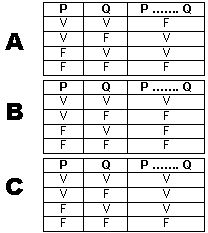
\includegraphics[width=0.28\textwidth]{mm11_connettivi}
\end{center}

Risultato: (A) XOR, (B) AND, (C) OR


\item [\nonumber]
\item {\bf A cosa serve il programma descritto dal seguente diagramma di flusso?}
\begin{center}
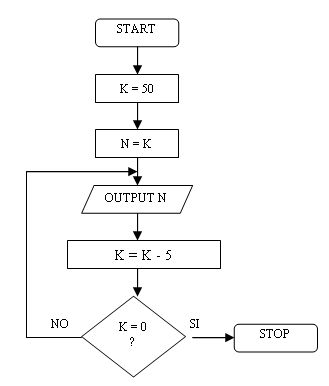
\includegraphics[width=0.45\textwidth]{mm4_fig5.jpg}
\end{center}

\item[$\square$]a dare in ouput 10 volte il numero 50


\item [\nonumber]
\item {\bf Che differenza esiste tra programma sorgente  ed un programma oggetto?}

\item[$\square$]Il programma sorgente \`{e} l'algoritmo scritto in un linguaggio ad alto livello mentre il programma oggetto \`{e} tradotto in linguaggio macchina
\

\item [\nonumber]
\item {\bf Quali sono gli input del linker?}
\item[$\square$] i file oggetto


\end{enumerate}



 

\end{document}
